% \clearpage
\section{Survey Questionnaire}\label{sec:app-survey}

This appendix contains the full text of the survey used in this study. The scenarios were assigned randomly. 

\subsection{Scenario 1 - Familiar}
Your friend is applying for a job and needs help. The company they are applying to uses an AI (Artificial Intelligence) tool that helps with hiring. The AI looks at two factors: the resume and the cover letter.

Right now, their score is 40 out of 100 on the resume and 60 out of 100 on the cover letter.

The company says each factor affects the final decision differently, as shown below in the graph.
\begin{figure}[ht]
    \centering
    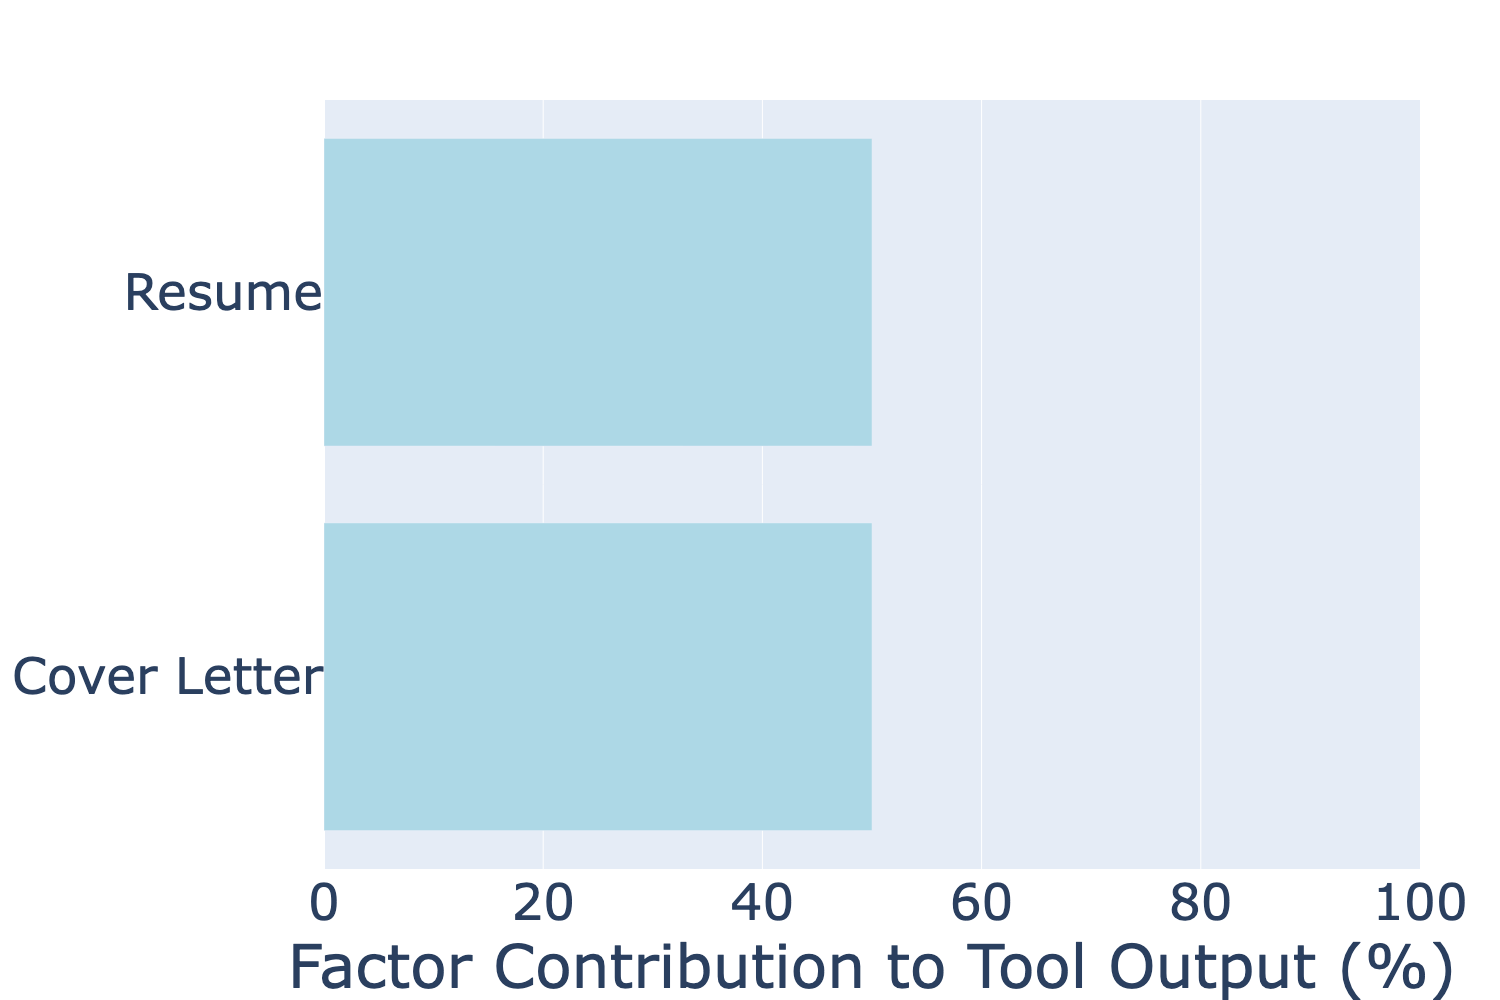
\includegraphics[width=0.4\textwidth]{Figures/2-equal.png}
    \caption{Feature weights for Scenario 1 - Familiar}
    \Description[Survey text for scenario 1 - Familiar]{The weights for scenario 1: Two features (equal)}
    \label{fig:survey-weights-scenario1}
\end{figure}

Your friend has 10 hours to get ready for the application. You want to help them decide how to use their time to improve their chances of getting a positive recommendation from the AI tool.

Your friend’s per-hour productivity rate in improving their score for each factor is as follows:
\begin{figure}[ht]
    \centering
    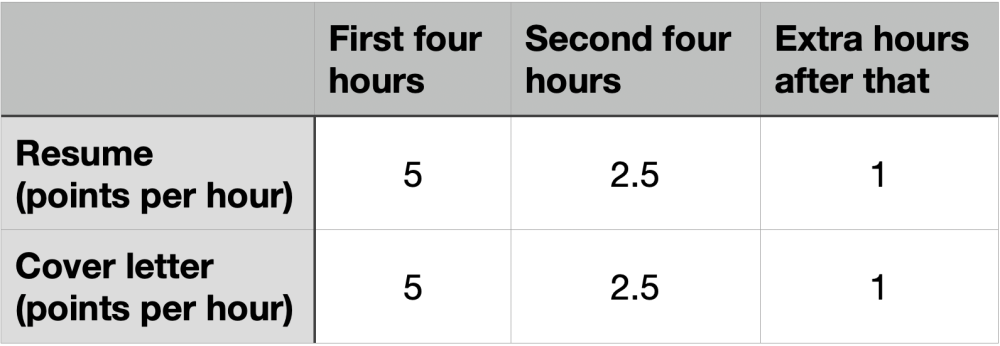
\includegraphics[width=0.5\textwidth]{Figures/cost-two.png}
    \caption{Productivity rate for Scenario 1}
    \Description[Survey text for scenario 1]{The cost description for two features}
    \label{fig:survey-cost-scenario1}
\end{figure}

The ten participants whose answers are closest to the best use of time will each receive a \$5 bonus.

\begin{itemize}
    \item Resume: \underline{\hspace{3cm}}
    \item Cover letter: \underline{\hspace{3cm}}
    \item Total: [Resume + Cover letter]
\end{itemize}


% \newpage
\subsection{Scenario 2 - Familiar}
Your friend is applying for a job and needs help. The company they are applying to uses an AI (Artificial Intelligence) tool that helps with hiring. The AI looks at two factors: the resume and the cover letter.

Right now, their score is 40 out of 100 on the resume and 60 out of 100 on the cover letter.

The company says each factor affects the final decision differently, as shown below in the graph.
\begin{figure}[ht]
    \centering
    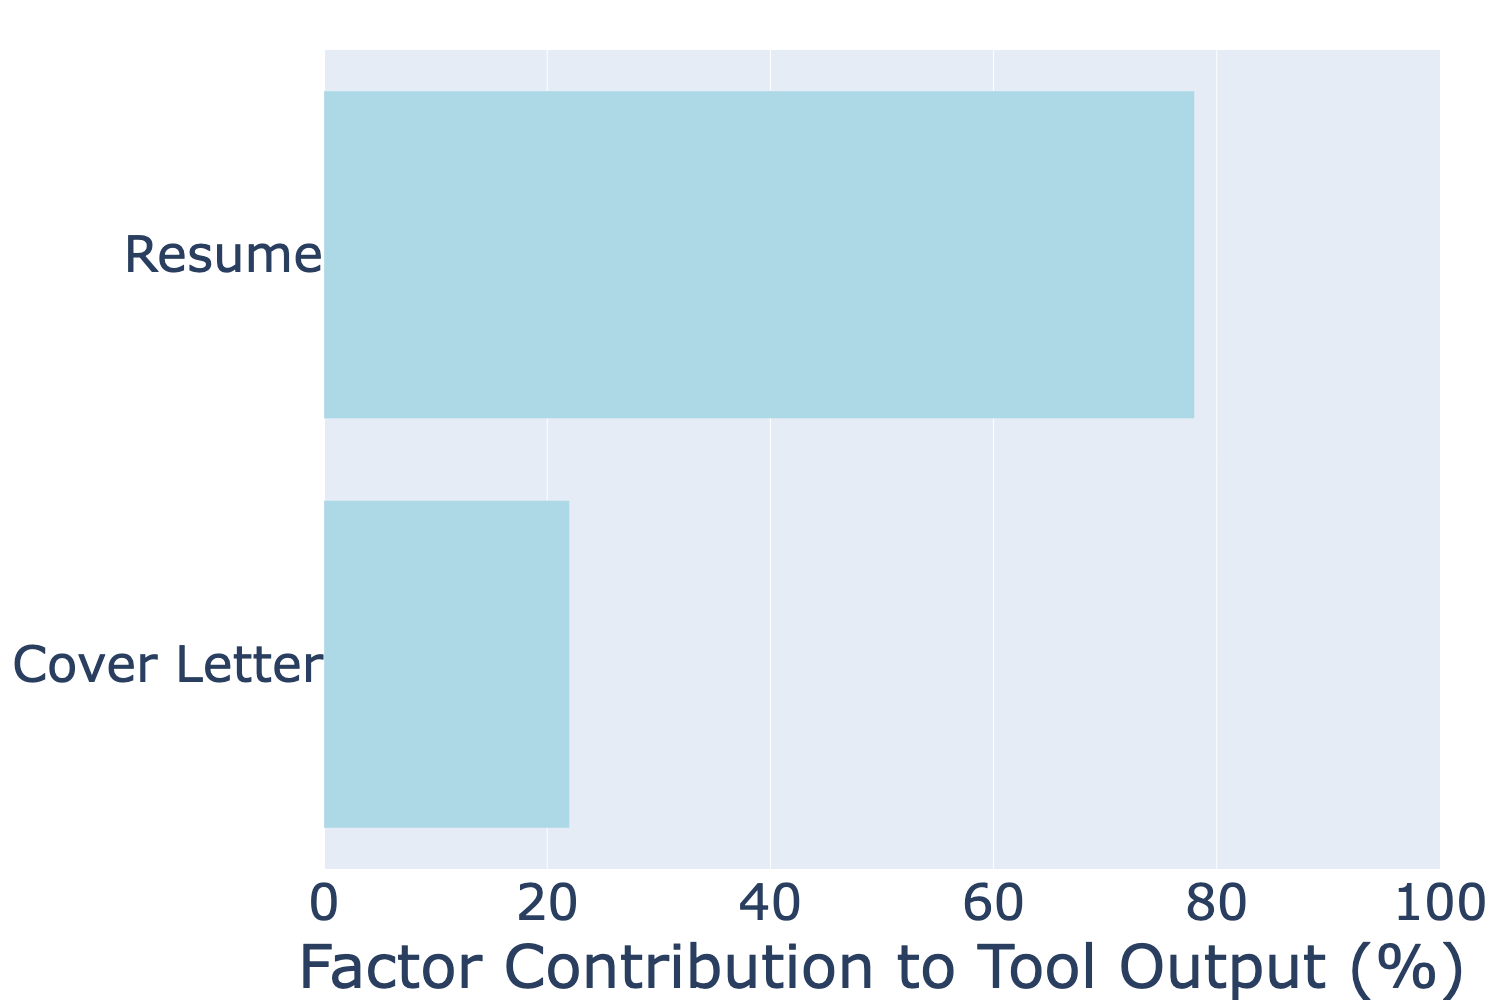
\includegraphics[width=0.4\textwidth]{Figures/2-unequal.png}
    \caption{Feature weights for Scenario 2 - Familiar}
    \Description[Survey text for scenario 2 - Familiar]{The weights for scenario 2: Two features (unequal)}
    \label{fig:survey-weights-scenario2}
\end{figure}

Your friend has 10 hours to get ready for the application. You want to help them decide how to use their time to improve their chances of getting a positive recommendation from the AI tool.

Your friend’s per-hour productivity rate in improving their score for each factor is as follows:
\begin{figure}[ht]
    \centering
    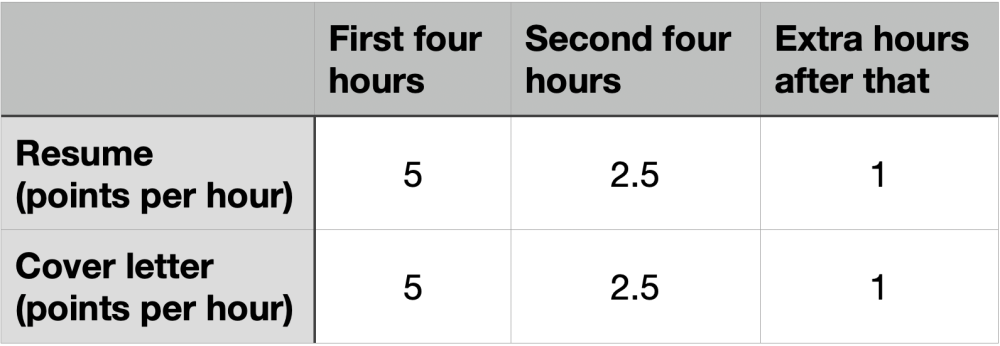
\includegraphics[width=0.5\textwidth]{Figures/cost-two.png}
    \caption{Productivity rate for Scenario 2 - Familiar}
    \Description[Survey text for scenario 2 - Familiar]{The cost description for two features}
    \label{fig:survey-cost-scenario2}
\end{figure}

The ten participants whose answers are closest to the best use of time will each receive a \$5 bonus.

\begin{itemize}
    \item Resume: \underline{\hspace{3cm}}
    \item Cover letter: \underline{\hspace{3cm}}
    \item Total: [Resume + Cover letter]
\end{itemize}


% \newpage
\subsection{Scenario 3 - Familiar}
Your friend is applying for a job and needs help. The company they are applying to uses an AI (Artificial Intelligence) tool that helps with hiring. The AI looks at four factors: the resume, the cover letter, LinkedIn profile, and on-site interview score.

Right now, their score is 60 out of 100 for on-site interview, 40 out of 100 on the resume, 60 out of 100 on the cover letter, and 65 out of 100 on the LinkedIn profile.

The company says each factor affects the final decision differently, as shown below in the graph.
\begin{figure}[ht]
    \centering
    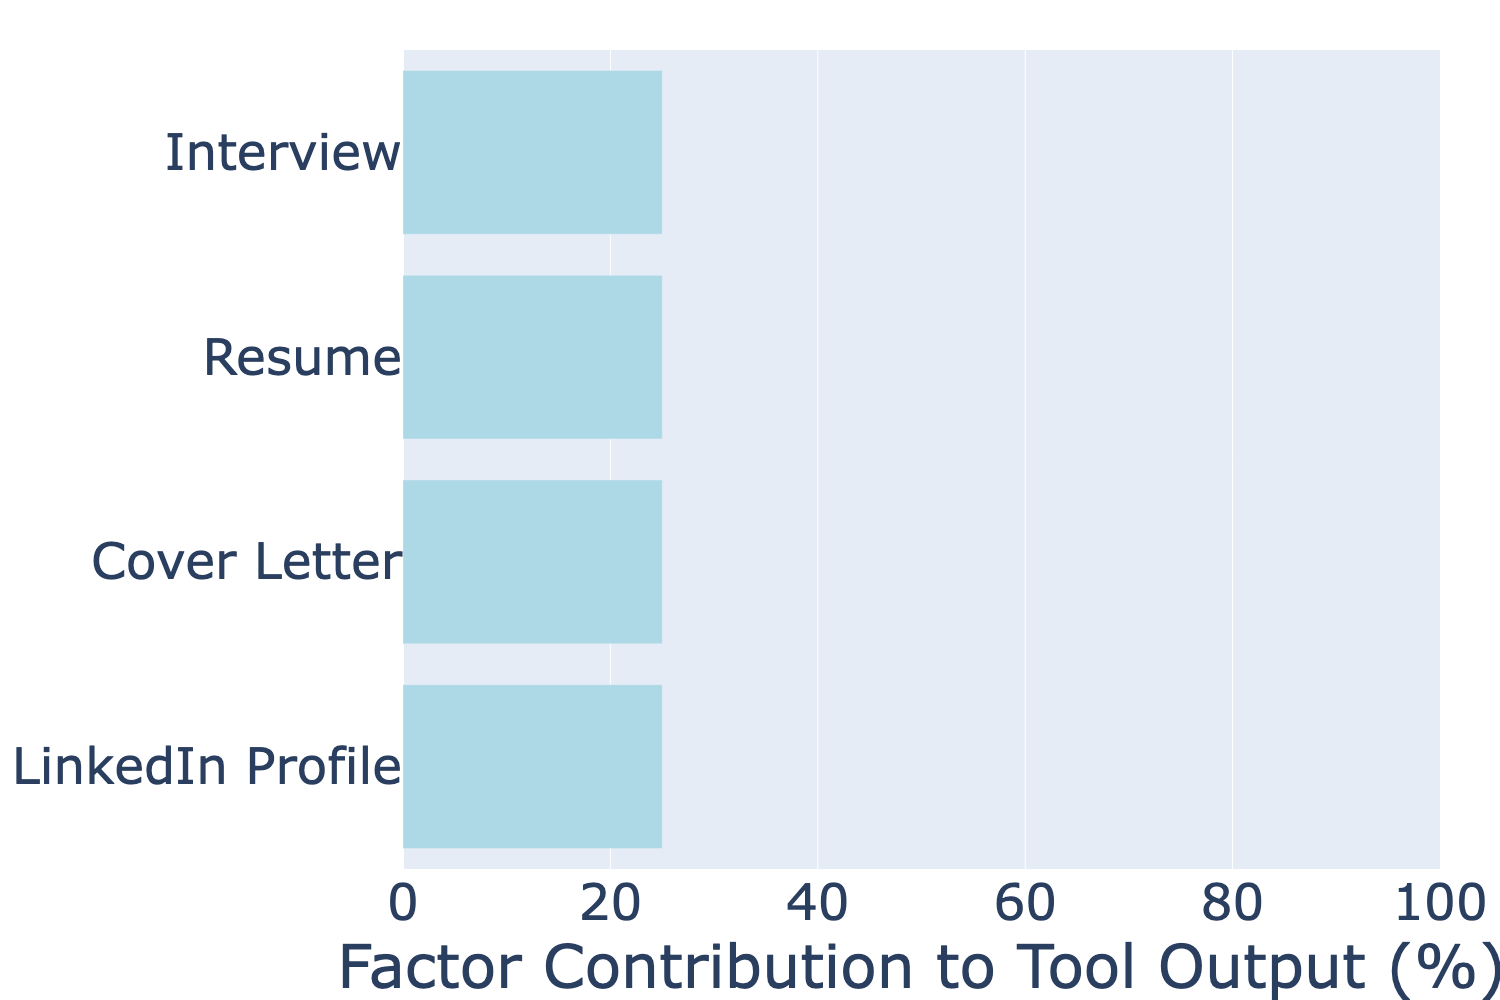
\includegraphics[width=0.4\textwidth]{Figures/4-equal.png}
    \caption{Feature weights for Scenario 3 - Familiar}
    \Description[Survey text for scenario 3 - Familiar]{The weights for scenario 3: Four features (equal)}
    \label{fig:survey-weights-scenario3}
\end{figure}

Your friend has 10 hours to get ready for the application. You want to help them decide how to use their time to improve their chances of getting a positive recommendation from the AI tool.

Your friend’s per-hour productivity rate in improving their score for each factor is as follows:
\begin{figure}[ht]
    \centering
    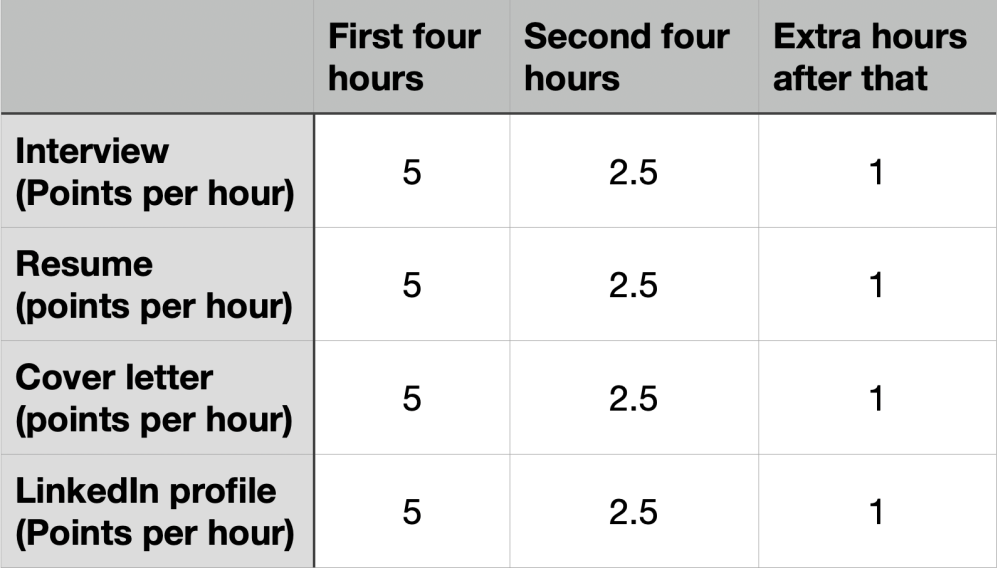
\includegraphics[width=0.4\textwidth]{Figures/cost-four.png}
    \caption{Productivity rate for Scenario 3 - Familiar}
    \Description[Survey text for scenario 3 - Familiar]{The cost description for four features}
    \label{fig:survey-cost-scenario3}
\end{figure}

The ten participants whose answers are closest to the best use of time will each receive a \$5 bonus.

\begin{itemize}
    \item Interview: \underline{\hspace{3cm}}
    \item Resume: \underline{\hspace{3cm}}
    \item Cover letter: \underline{\hspace{3cm}}
    \item LinkedIn profile: \underline{\hspace{3cm}}
    \item Total: [Interview + Resume + Cover letter + LinkedIn profile]
\end{itemize}


% \newpage
\subsection{Scenario 4 - Familiar}
Your friend is applying for a job and needs help. The company they are applying to uses an AI (Artificial Intelligence) tool that helps with hiring. The AI looks at four factors: the resume, the cover letter, LinkedIn profile, and on-site interview score.

Right now, their score is 60 out of 100 for on-site interview, 40 out of 100 on the resume, 60 out of 100 on the cover letter, and 65 out of 100 on the LinkedIn profile.

The company says each factor affects the final decision differently, as shown below in the graph.
\begin{figure}[ht]
    \centering
    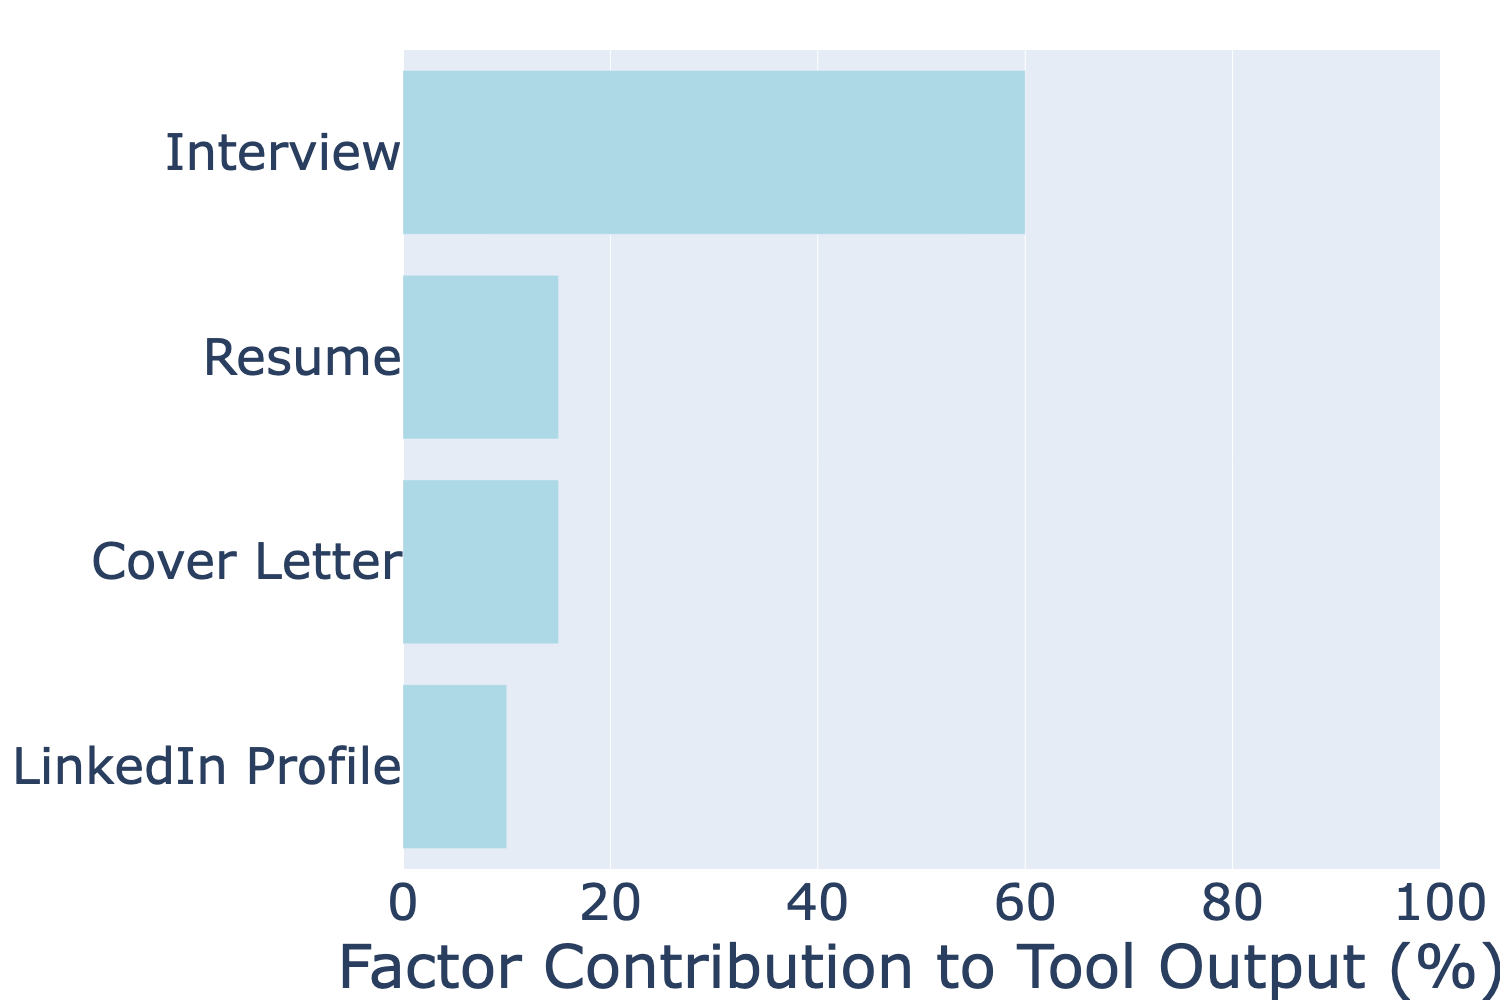
\includegraphics[width=0.4\textwidth]{Figures/4-unequal.png}
    \caption{Feature weights for Scenario 4 - Familiar}
    \Description[Survey text for scenario 4 - Familiar]{The weights for scenario 4: Four features (unequal)}
    \label{fig:survey-weights-scenario4}
\end{figure}

Your friend has 10 hours to get ready for the application. You want to help them decide how to use their time to improve their chances of getting a positive recommendation from the AI tool.

Your friend’s per-hour productivity rate in improving their score for each factor is as follows:
\begin{figure}[ht]
    \centering
    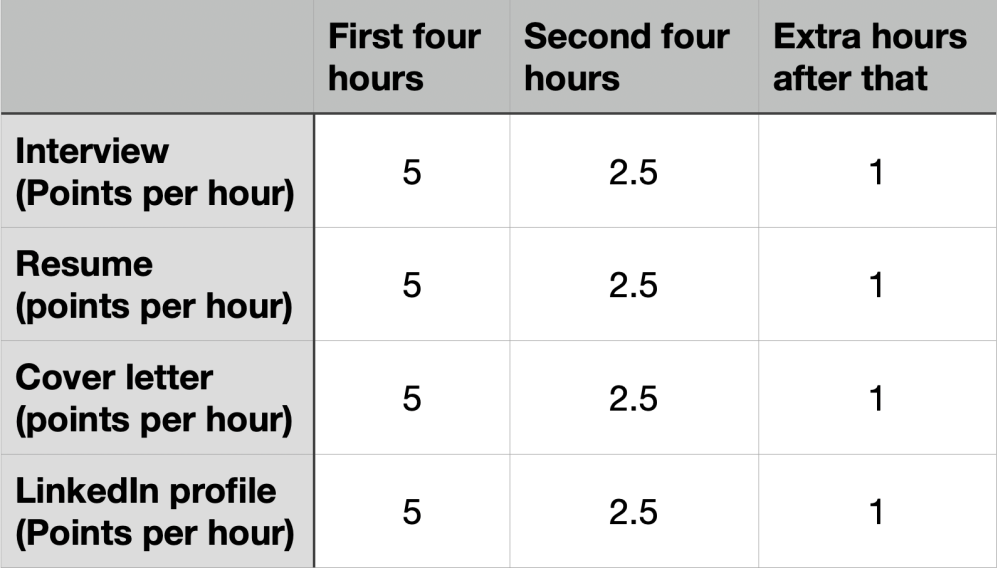
\includegraphics[width=0.4\textwidth]{Figures/cost-four.png}
    \caption{Productivity rate for Scenario 4 - Familiar}
    \Description[Survey text for scenario 4 - Familiar]{The cost description for four features}
    \label{fig:survey-cost-scenario4}
\end{figure}

The ten participants whose answers are closest to the best use of time will each receive a \$5 bonus.

\begin{itemize}
    \item Interview: \underline{\hspace{3cm}}
    \item Resume: \underline{\hspace{3cm}}
    \item Cover letter: \underline{\hspace{3cm}}
    \item LinkedIn profile: \underline{\hspace{3cm}}
    \item Total: [Interview + Resume + Cover letter + LinkedIn profile]
\end{itemize}


% \subsection{Satisfaction}
% \begin{enumerate}
%     \item The system was easy to use
%     \begin{itemize}
%         \item[ ] Extremely difficult (1)
%         \item[ ] Somewhat difficult (2)
%         \item[ ] Neither easy nor difficult (3)
%         \item[ ] Somewhat easy (4)
%         \item[ ] Extremely easy (5)
%     \end{itemize}
    
%     \item The explanation of how the tool works was useful for my goals
%     \begin{itemize}
%         \item[ ] Strongly disagree (1)
%         \item[ ] Somewhat disagree (2)
%         \item[ ] Neither agree nor disagree (3)
%         \item[ ] Somewhat agree (4)
%         \item[ ] Strongly agree (5)
%     \end{itemize}

%     \item Rate your satisfaction with the explanation
%     \begin{itemize}
%         \item[ ] Extremely dissatisfied (1)
%         \item[ ] Somewhat dissatisfied (2)
%         \item[ ] Neither satisfied nor dissatisfied (3)
%         \item[ ] Somewhat satisfied (4)
%         \item[ ] Extremely satisfied (5)
%     \end{itemize}
% \end{enumerate}

% \subsection{Understanding}
% \begin{enumerate}
%     \item I understand the explanation of how the tool works
%     \begin{itemize}
%         \item[ ] Not well at all (1)
%         \item[ ] Slightly well (2)
%         \item[ ] Moderately well (3)
%         \item[ ] Very well (4)
%         \item[ ] Extremely well (5)
%     \end{itemize}
    
%     \item How confident are you in your answer
%     \begin{itemize}
%         \item[ ] Very confident (1)
%         \item[ ] Somewhat confident (2)
%         \item[ ] Neither confident nor unsure (3)
%         \item[ ] Somewhat unsure (4)
%         \item[ ] Very unsure (5)
%     \end{itemize}

%     \item Assume the organization's tool gives the following weights: Resume (70\%) and cover letter (30\%) A person has a score of 50 out of 100 for resume and 50 out of 100 for cover letter. They spend all their time to improve their cover letter. Is this the best use of their time?
%     \begin{itemize}
%         \item[ ] Yes
%         \item[ ] No
%     \end{itemize}
% \end{enumerate}

% \subsection{Trust}
% \begin{enumerate}
%     \item Do you think that the system is trustworthy?
%     \begin{itemize}
%         \item[ ] Very safe (1)
%         \item[ ] Somewhat safe (2)
%         \item[ ] Neither safe nor unsafe (3)
%         \item[ ] Somewhat dangerous (4)
%         \item[ ] Very dangerous (5)
%     \end{itemize}
    
%     \item Is the tool efficient at what is does?
%     \begin{itemize}
%         \item[ ] Definitely not (1)
%         \item[ ] Probably not (2)
%         \item[ ] Might or might not (3)
%         \item[ ] Probably yes (4)
%         \item[ ] Definitely yes (5)
%     \end{itemize}

%     \item What is your confidence in the tool?
%     \begin{itemize}
%         \item[ ] None at all (1)
%         \item[ ] A little (2) 
%         \item[ ] A moderate amount (3)
%         \item[ ] A lot (4)
%         \item[ ] A great deal (5)
%     \end{itemize}
% \end{enumerate}

% \subsection{Task Performance}
% \begin{enumerate}
%     \item How difficult was the task?
%     \begin{itemize}
%         \item[ ] Extremely difficult (1)
%         \item[ ] Somewhat difficult (2)
%         \item[ ] Neither easy nor difficult (3)
%         \item[ ] Somewhat easy (4)
%         \item[ ] Extremely easy (5)
%     \end{itemize}
    
%     \item How successful were you at the task?
%     \begin{itemize}
%         \item[ ] Very unsuccessful (1)
%         \item[ ] Somewhat unsuccessful (2)
%         \item[ ] Neither successful not unsuccessful (3)
%         \item[ ] Somewhat successful (4)
%         \item[ ] Very successful (5)
%     \end{itemize}

%     \item How mentally demanding was the task?
%     \begin{itemize}
%         \item[ ] Very low (1)
%         \item[ ] Somewhat low (2)
%         \item[ ] Neither low nor high (3)
%         \item[ ] Somewhat high (4)
%         \item[ ] Very high (5)
%     \end{itemize}
% \end{enumerate}

% \subsection{Tech Familiarity}
% How familiar are you with the following computer and internet related items? Please don't look up anything about the terms below, as we want to know your responses based on the information you already have.
% \begin{table}[ht]
% \caption{} 
% \begin{center}
%     \begin{tabular}{llllll}
%     & \thead{Not familiar \\ at all}  & \thead{Slightly\\ familiar} & \thead{Moderately\\ familiar} & \thead{Very\\ familiar} & \thead{Extremely\\ familiar} \\
%     \hline
%     \makecell{Backpropagation} \\
%     \makecell{k-Nearest Neighbors (KNN)} \\
%     \makecell{Citrus++} \\
%     \makecell{Support Vector Machines (SVM)} \\
%     \makecell{Data Reversion} \\
%     \makecell{PyCharm} \\
%     \end{tabular}
% \end{center}
% \end{table}

% \subsection{Demographics}
% Please state your gender
% \begin{itemize}
%     \item Male
%     \item Female
%     \item Non-binary / gender non-conforming
%     \item Prefer not to say
%     \item Prefer to self-describe: \underline{\hspace{3cm}}
% \end{itemize}

% How old are you? (e.g. 19) \underline{\hspace{3cm}}

% Please state your ethnicity
% \begin{itemize}
%     \item American Indian, Alaska native
%     \item Asian
%     \item Black, African American
%     \item Hispanic, Latino, or Spanish
%     \item Middle Eastern and North African Native Hawaiian or Other Pacific Islander 
%     \item White
%     \item Prefer not to say
% \end{itemize}

% What is the highest level of education you have completed?
% \begin{itemize}
%     \item Less than a high school diploma
%     \item High school degree or equivalent (e.g. GED)
%     \item Technical, trade or vocational school AFTER high school
%     \item Some college, no degree
%     \item 2 year college (e.g. AA, AS)
%     \item 4 year college (e.g. BA, BS)
%     \item Prefer not to say
% \end{itemize}
% \newpage
\subsection{Scenario 1 - Unfamiliar}
Your friend has been diagnosed with Coronary Artery Disease (CAD) and needs to improve their health metrics to reduce the risk of a future heart attack. Their cardiologist uses an AI (Artificial Intelligence) tool to assess the likelihood of a major cardiovascular event. The AI evaluates four key health factors: LDL cholesterol (low-density lipoprotein), VO2 max (aerobic fitness), arterial stiffness index, and inflammatory markers (C-reactive protein, CRP).

Currently, their scores are as follows (higher score means healthier):
\begin{itemize}
    \item LDL Cholesterol: 60 out of 100
    \item VO2 Max: 40 out of 100
    \item Arterial Stiffness Index: 60 out of 100
    \item Inflammatory Markers: 65 out of 100
\end{itemize}

Each factor has a different weight in the AI’s calculation, as shown in the graph below. Some factors are more critical than others for reducing overall risk.
\begin{figure}[ht]
    \centering
    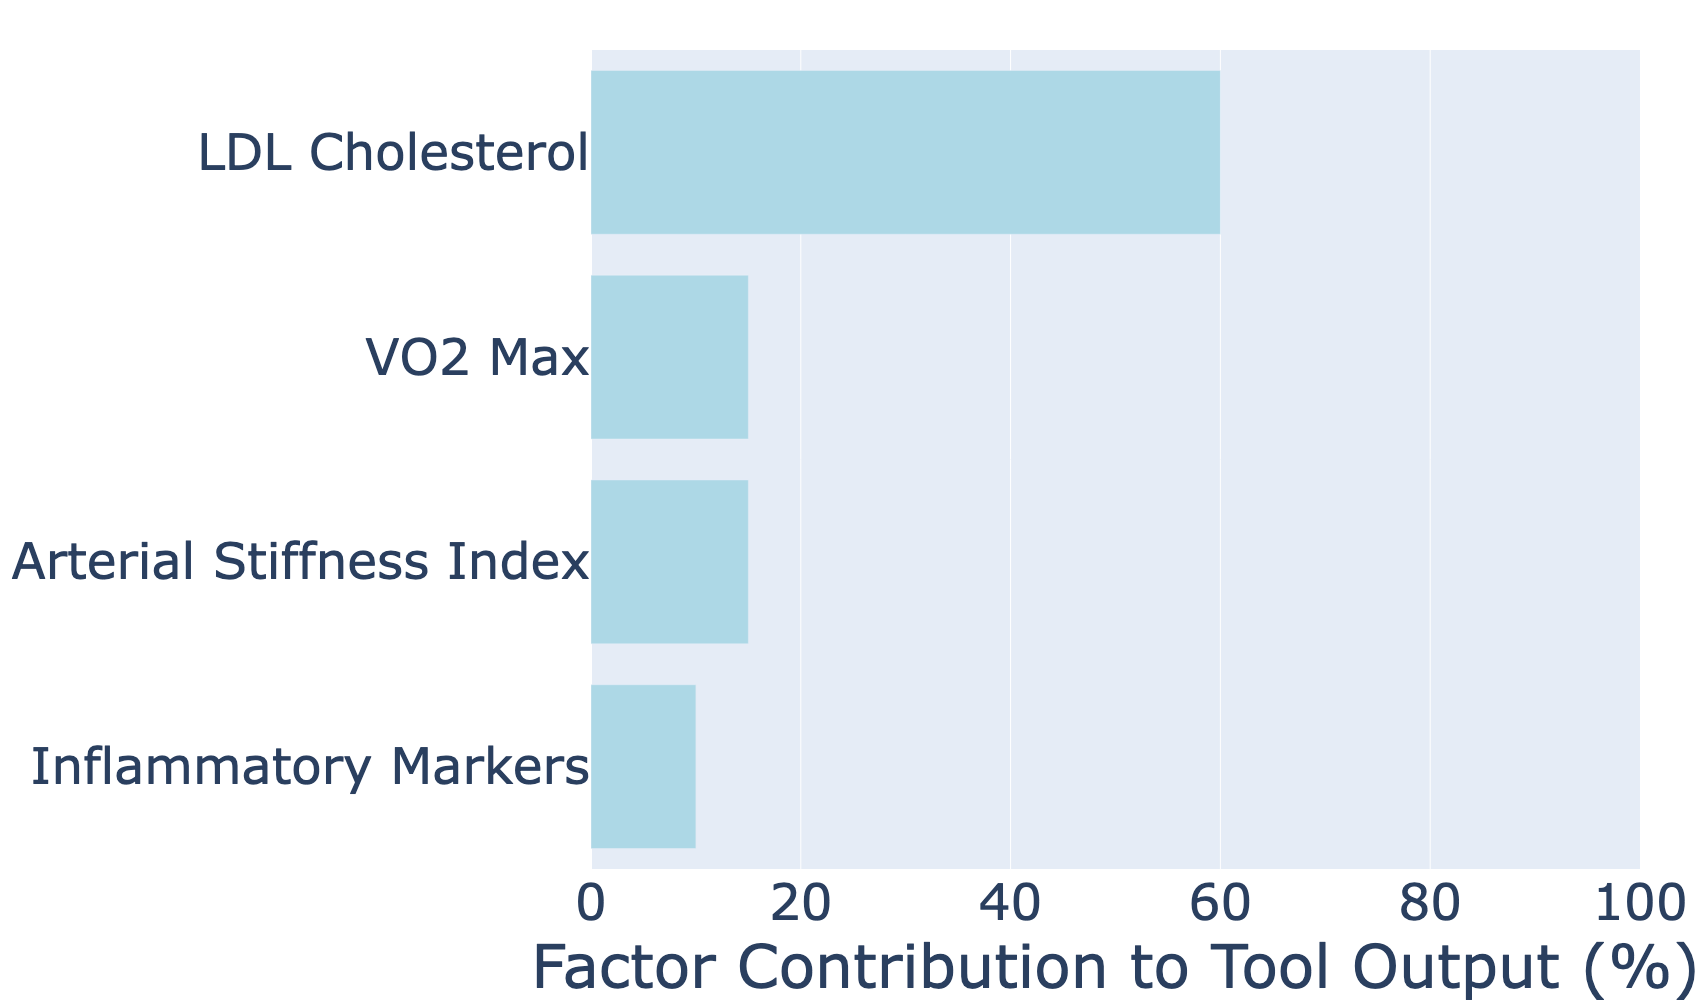
\includegraphics[width=0.4\textwidth]{Figures/4_unf_unbal.png}
    \caption{Feature weights for Scenario 1 - Unfamiliar}
    \Description[Survey text for scenario 1 - Unfamiliar]{The weights for scenario 1: 4 features (unequal)}
    \label{fig:survey-weights-scenario1-unf}
\end{figure}

Your friend has 10 weeks to improve these scores before their next check-up. You want to help them decide how to allocate their time and efforts to reduce their risk of a cardiovascular event.

Your friend’s per-hour productivity rate in improving their score for each factor is as follows:

\begin{figure}[ht]
    \centering
    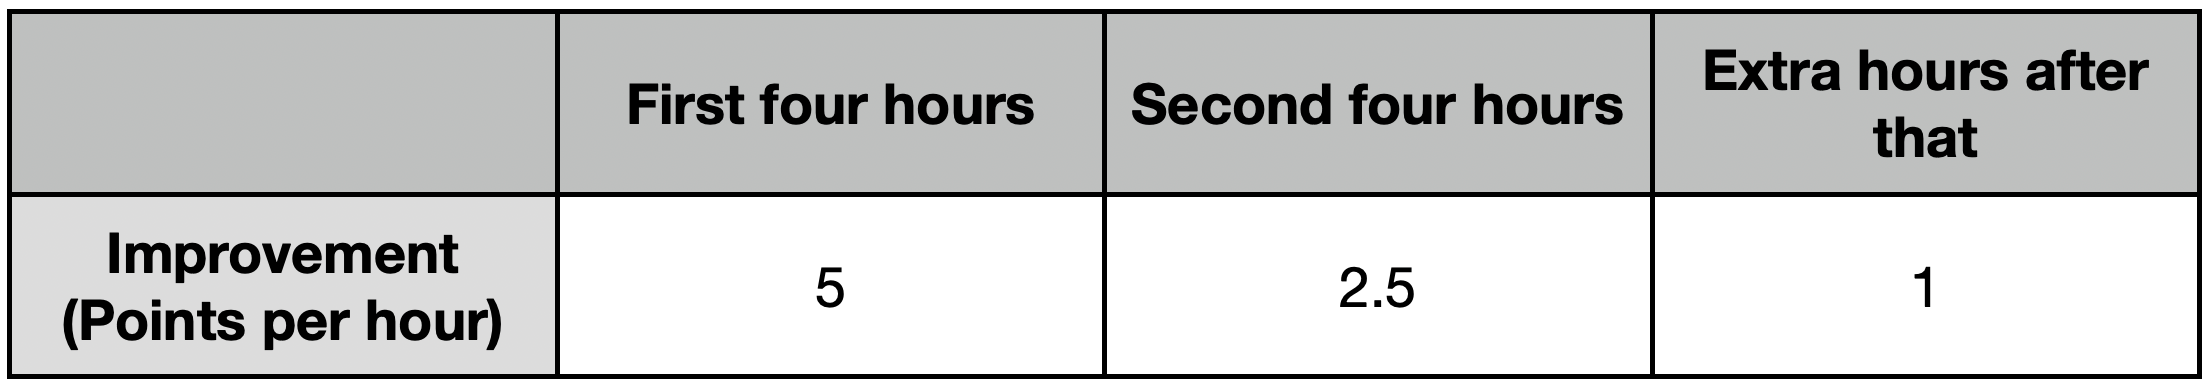
\includegraphics[width=0.5\textwidth]{Figures/rate-unf.png}
    \caption{Productivity rate for Scenario 1 - Unfamiliar}
    \Description[Survey text for scenario 1 - Unfamiliar]{The cost description}
    \label{fig:survey-cost-scenario1-unf}
\end{figure}

Based on this, how should your friend use their 10 weeks improving the factors to maximize their chances of a healthy outcome?

The ten participants whose answers are closest to the best use of time will each receive a \$5 bonus. 

\begin{itemize}
    \item LDL cholesterol (diet): \underline{\hspace{2cm}}
    \item VO2 max (exercise): \underline{\hspace{2cm}}
    \item Arterial Stiffness Index (yoga and medications): \underline{\hspace{2cm}}
    \item Inflammatory Markers (stress and sleep): \underline{\hspace{2cm}}
    \item Total: [VO2 max + LDL cholesterol + Arterial Stiffness Index + Inflammatory Markers]
\end{itemize}

% \newpage
\subsection{Scenario 2 - Unfamiliar}
Your friend has been diagnosed with Coronary Artery Disease (CAD) and needs to improve their health metrics to reduce the risk of a future heart attack. Their cardiologist uses an AI (Artificial Intelligence) tool to assess the likelihood of a major cardiovascular event. The AI evaluates four key health factors: LDL cholesterol (low-density lipoprotein), VO2 max (aerobic fitness), arterial stiffness index, and inflammatory markers (C-reactive protein, CRP).

Currently, their scores are as follows (higher score means healthier):
\begin{itemize}
    \item LDL Cholesterol: 60 out of 100
    \item VO2 Max: 40 out of 100
    \item Arterial Stiffness Index: 60 out of 100
    \item Inflammatory Markers: 65 out of 100
\end{itemize}

Each factor has a different weight in the AI’s calculation, as shown in the graph below. Some factors are more critical than others for reducing overall risk.
\begin{figure}[ht]
    \centering
    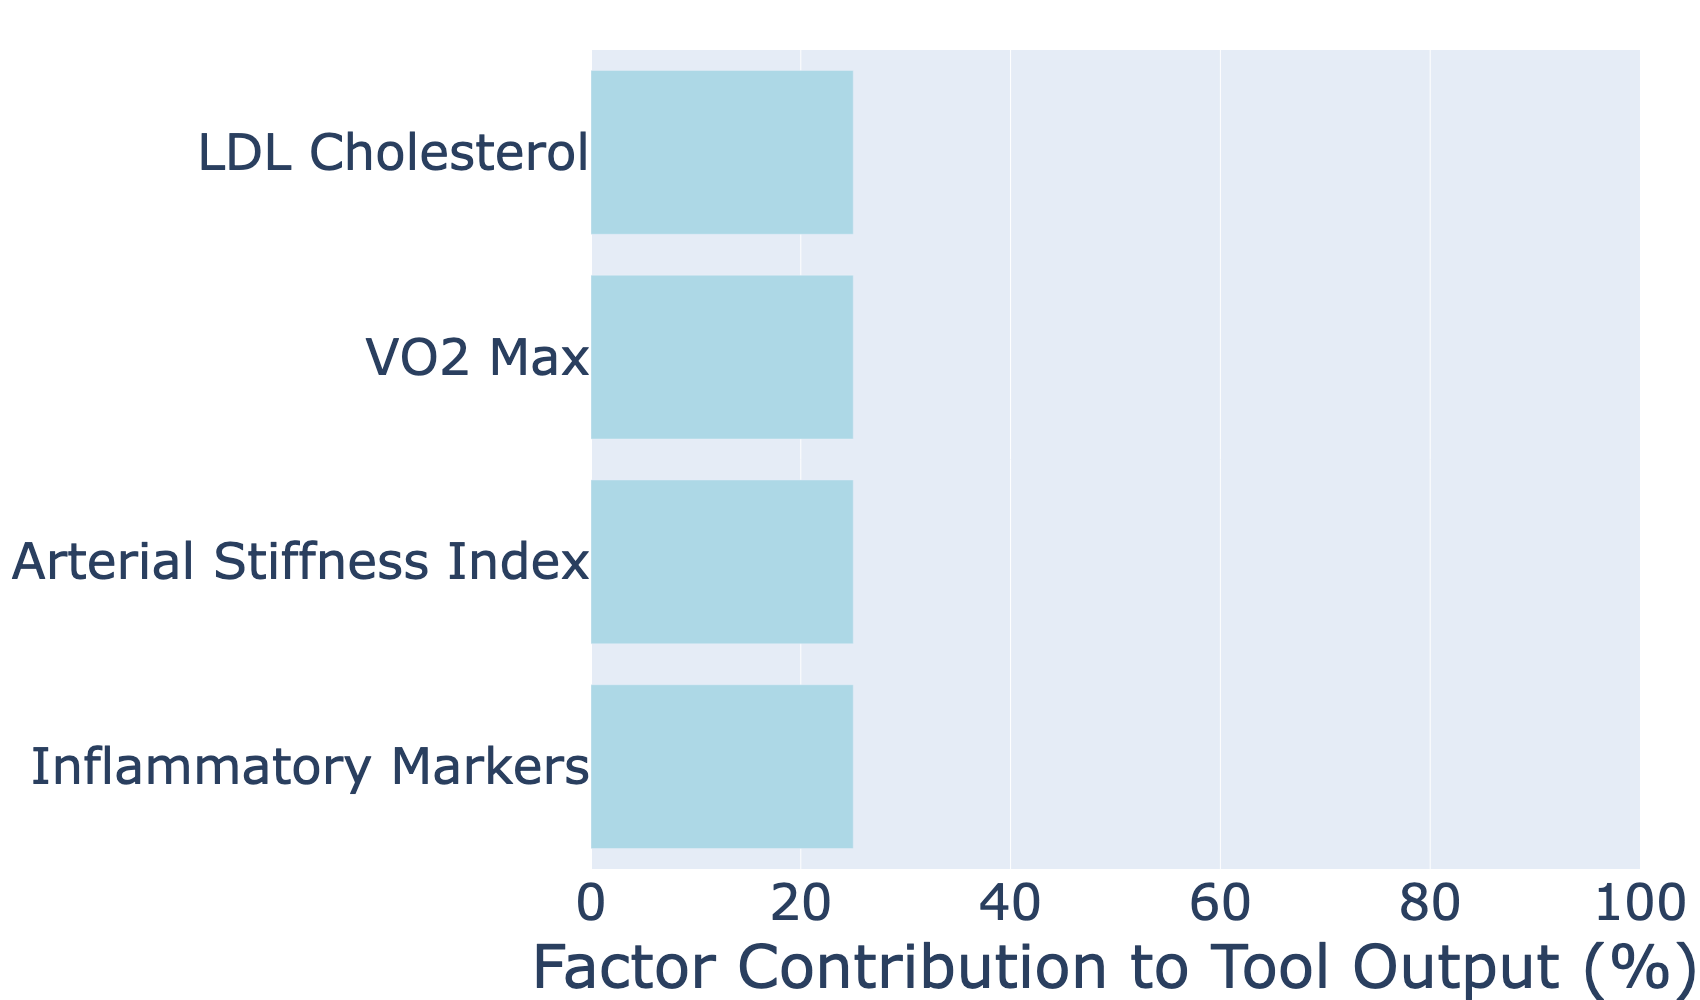
\includegraphics[width=0.4\textwidth]{Figures/4_unf_bal.png}
    \caption{Feature weights for Scenario 2 - Unfamiliar}
    \Description[Survey text for scenario 2 - Unfamiliar]{The weights for scenario 1: 4 features (equal)}
    \label{fig:survey-weights-scenario2-unf}
\end{figure}

Your friend has 10 weeks to improve these scores before their next check-up. You want to help them decide how to allocate their time and efforts to reduce their risk of a cardiovascular event.

Your friend’s per-hour productivity rate in improving their score for each factor is as follows:

\begin{figure}[ht]
    \centering
    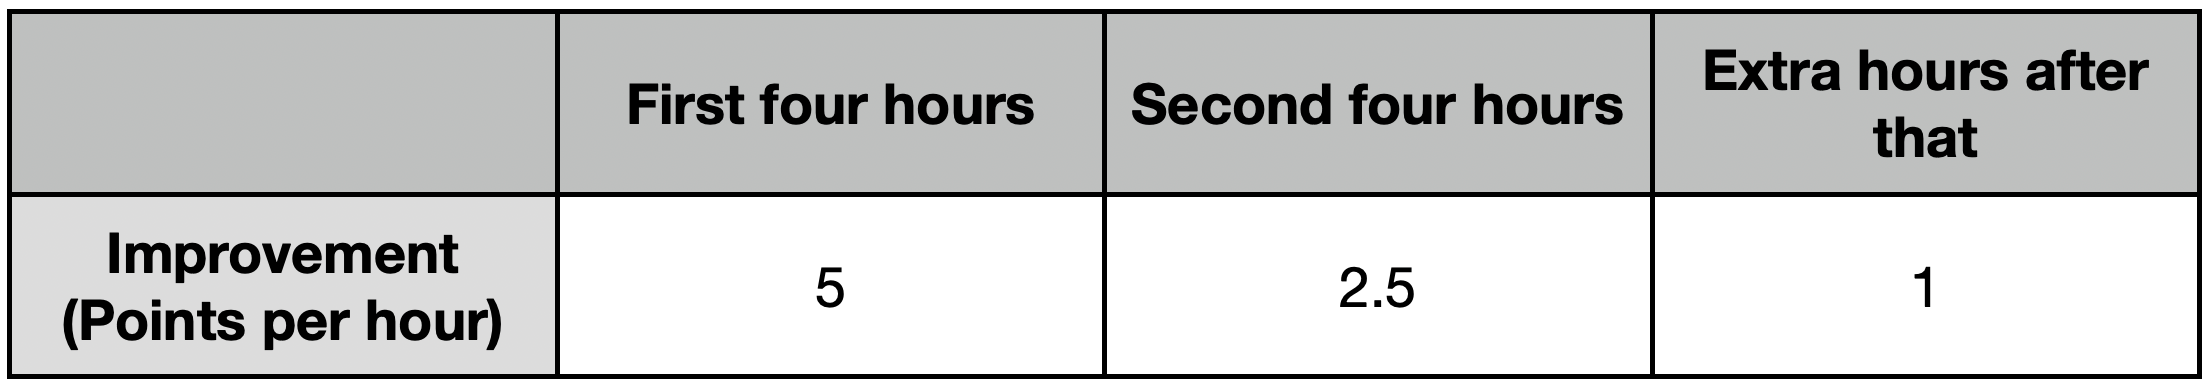
\includegraphics[width=0.5\textwidth]{Figures/rate-unf.png}
    \caption{Productivity rate for Scenario 2 - Unfamiliar}
    \Description[Survey text for scenario 2 - Unfamiliar]{The cost description}
    \label{fig:survey-cost-scenario2-unf}
\end{figure}

Based on this, how should your friend use their 10 weeks improving the factors to maximize their chances of a healthy outcome?

The ten participants whose answers are closest to the best use of time will each receive a \$5 bonus. 

\begin{itemize}
    \item LDL cholesterol (diet): \underline{\hspace{2cm}}
    \item VO2 max (exercise): \underline{\hspace{2cm}}
    \item Arterial Stiffness Index (yoga and medications): \underline{\hspace{2cm}}
    \item Inflammatory Markers (stress and sleep): \underline{\hspace{2cm}}
    \item Total: [VO2 max + LDL cholesterol + Arterial Stiffness Index + Inflammatory Markers]
\end{itemize}

% \newpage
\subsection{Scenario 3 - Unfamiliar}
Your friend has been diagnosed with Coronary Artery Disease (CAD) and needs to improve their health metrics to reduce the risk of a future heart attack. Their cardiologist uses an AI (Artificial Intelligence) tool to assess the likelihood of a major cardiovascular event. The AI evaluates two key health factors: LDL cholesterol (low-density lipoprotein) and VO2 max (aerobic fitness).

Currently, their scores are as follows (higher score means healthier):
\begin{itemize}
    \item LDL Cholesterol: 60 out of 100
    \item VO2 Max: 40 out of 100
\end{itemize}

Each factor has a different weight in the AI’s calculation, as shown in the graph below. Some factors are more critical than others for reducing overall risk.
\begin{figure}[ht]
    \centering
    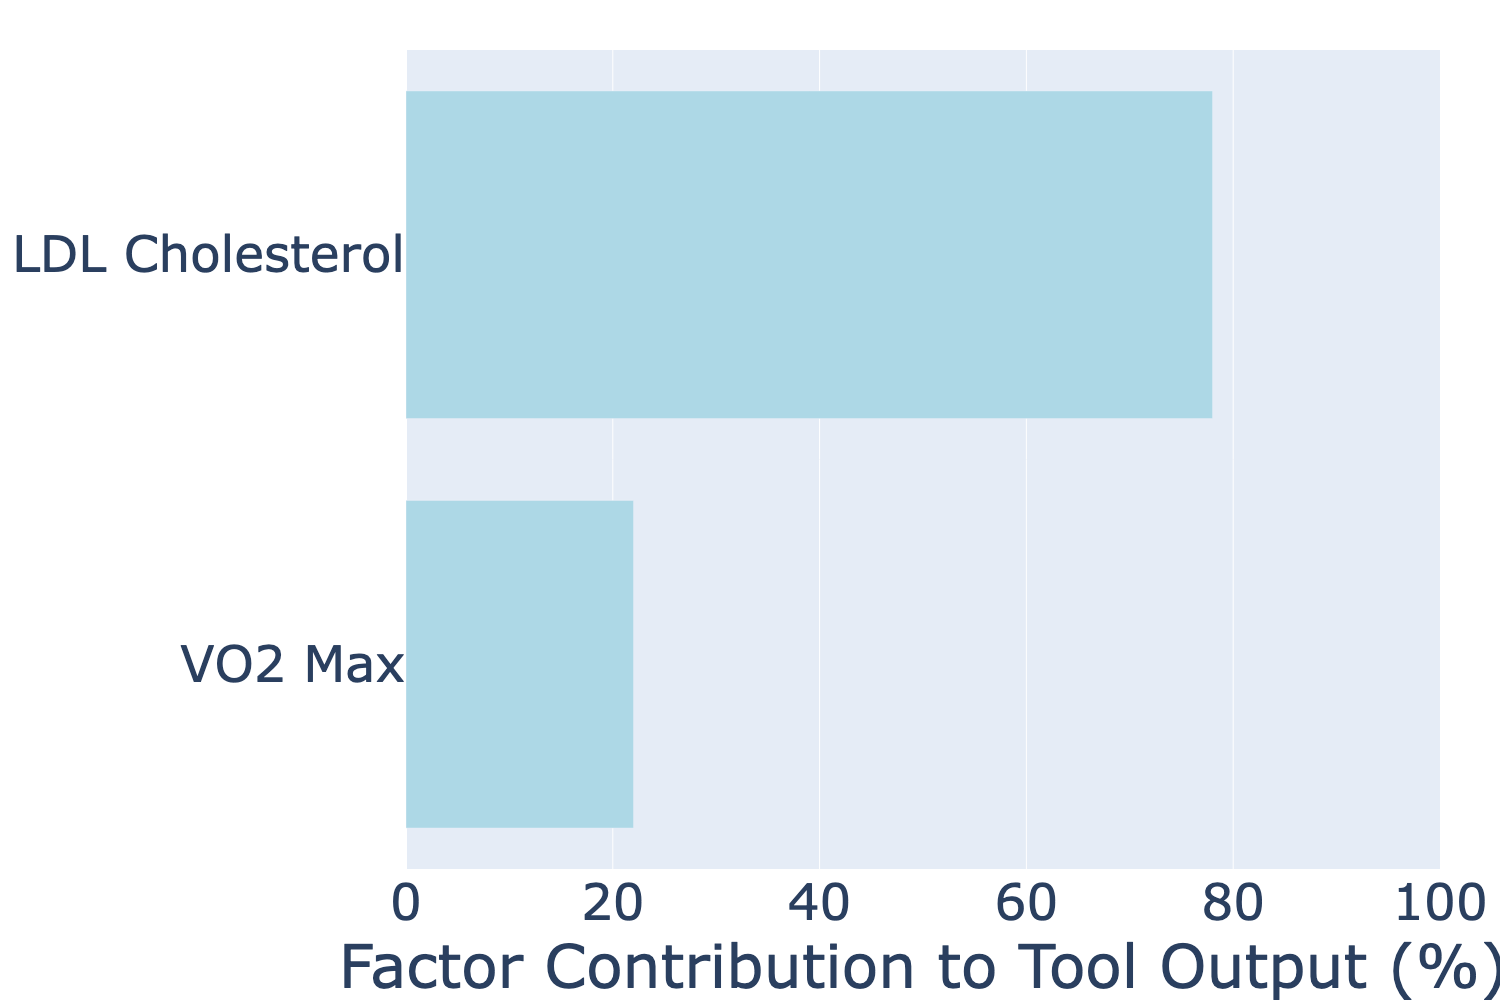
\includegraphics[width=0.4\textwidth]{Figures/2_unf_unbal.png}
    \caption{Feature weights for Scenario 3 - Unfamiliar}
    \Description[Survey text for scenario 3 - Unfamiliar]{The weights for scenario 1: 2 features (unequal)}
    \label{fig:survey-weights-scenario3-unf}
\end{figure}

Your friend has 10 weeks to improve these scores before their next check-up. You want to help them decide how to allocate their time and efforts to reduce their risk of a cardiovascular event.

Your friend’s per-hour productivity rate in improving their score for each factor is as follows:

\begin{figure}[ht]
    \centering
    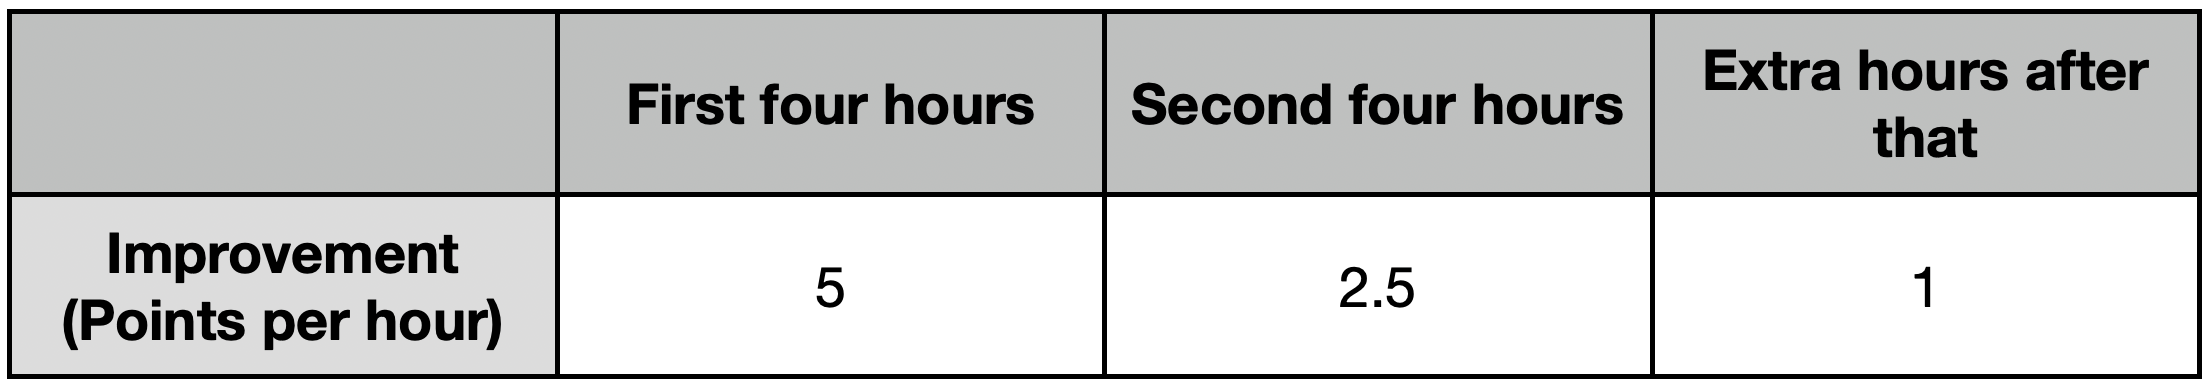
\includegraphics[width=0.4\textwidth]{Figures/rate-unf.png}
    \caption{Productivity rate for Scenario 3 - Unfamiliar}
    \Description[Survey text for scenario 3 - Unfamiliar]{The cost description}
    \label{fig:survey-cost-scenario3-unf}
\end{figure}

Based on this, how should your friend use their 10 weeks improving the factors to maximize their chances of a healthy outcome?

The ten participants whose answers are closest to the best use of time will each receive a \$5 bonus. 

\begin{itemize}
    \item LDL cholesterol (diet): \underline{\hspace{3cm}}
    \item VO2 max (exercise): \underline{\hspace{3cm}}
    \item Total: [VO2 max + LDL cholesterol]
\end{itemize}

% \newpage
\subsection{Scenario 4 - Unfamiliar}
Your friend has been diagnosed with Coronary Artery Disease (CAD) and needs to improve their health metrics to reduce the risk of a future heart attack. Their cardiologist uses an AI (Artificial Intelligence) tool to assess the likelihood of a major cardiovascular event. The AI evaluates two key health factors: LDL cholesterol (low-density lipoprotein) and VO2 max (aerobic fitness).

Currently, their scores are as follows (higher score means healthier):
\begin{itemize}
    \item LDL Cholesterol: 60 out of 100
    \item VO2 Max: 40 out of 100
\end{itemize}

Each factor has a different weight in the AI’s calculation, as shown in the graph below. Some factors are more critical than others for reducing overall risk.
\begin{figure}[ht]
    \centering
    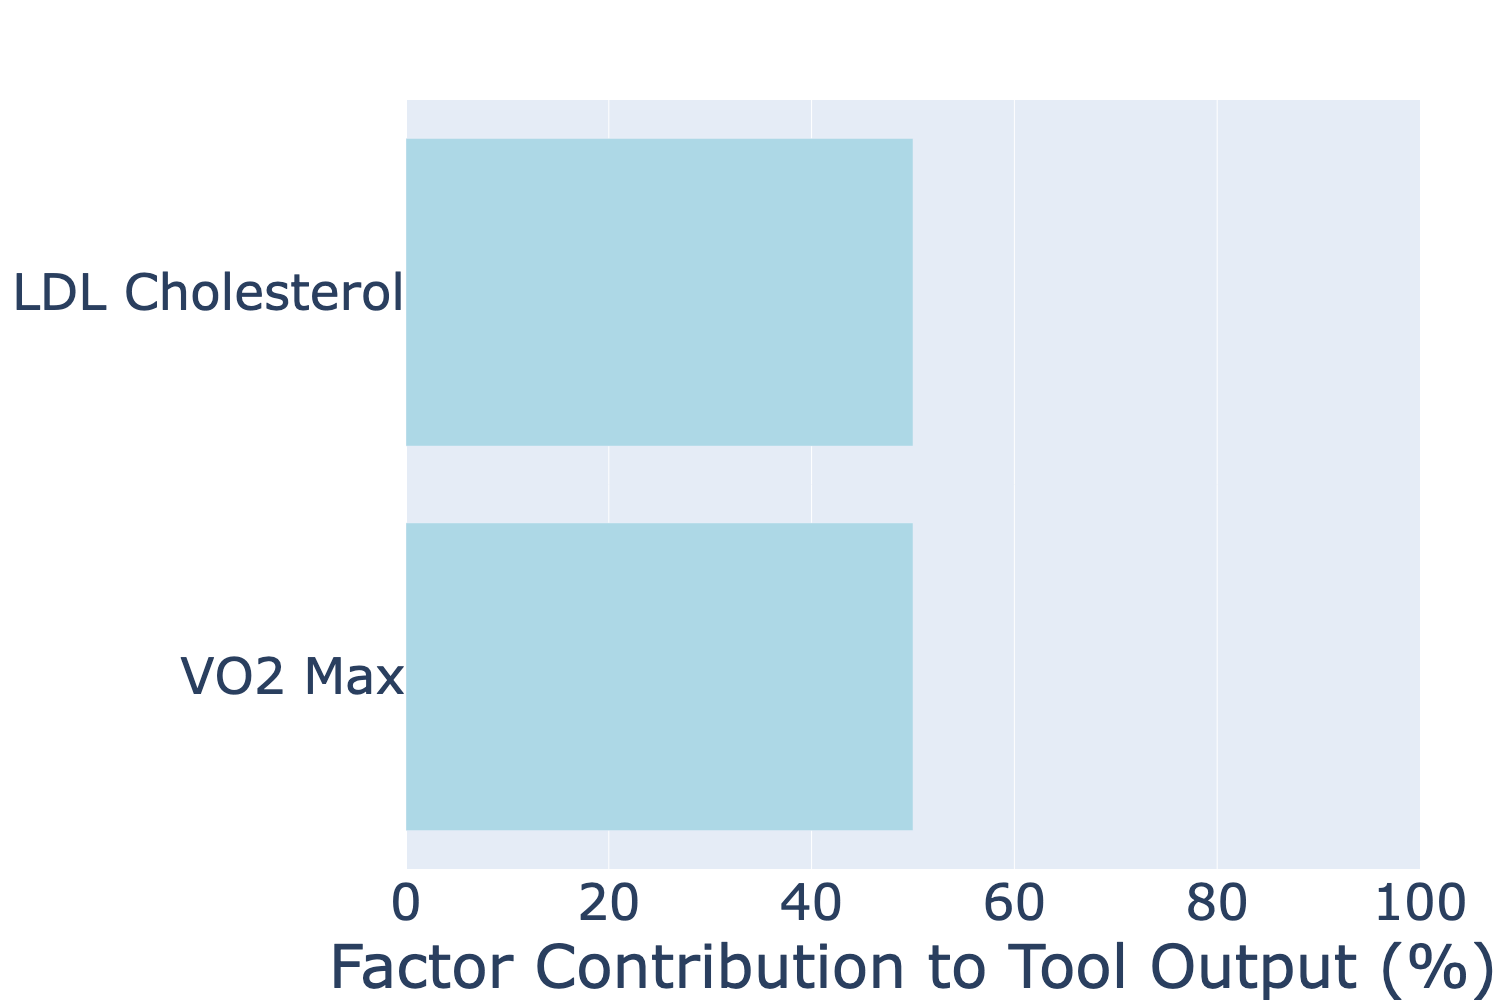
\includegraphics[width=0.4\textwidth]{Figures/2_unf_bal.png}
    \caption{Feature weights for Scenario 4 - Unfamiliar}
    \Description[Survey text for scenario 4 - Unfamiliar]{The weights for scenario 1: 2 features (equal)}
    \label{fig:survey-weights-scenario4-unf}
\end{figure}

Your friend has 10 weeks to improve these scores before their next check-up. You want to help them decide how to allocate their time and efforts to reduce their risk of a cardiovascular event.

Your friend’s per-hour productivity rate in improving their score for each factor is as follows:

\begin{figure}[ht]
    \centering
    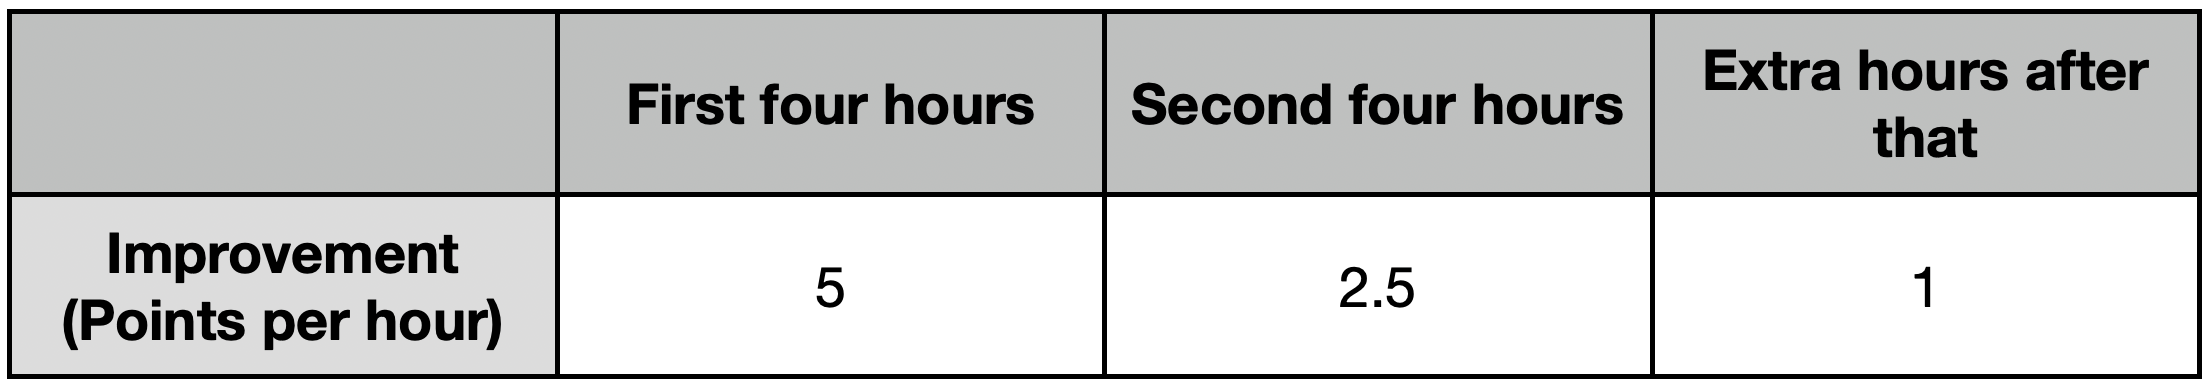
\includegraphics[width=0.5\textwidth]{Figures/rate-unf.png}
    \caption{Productivity rate for Scenario 4 - Unfamiliar}
    \Description[Survey text for scenario 4 - Unfamiliar]{The cost description}
    \label{fig:survey-cost-scenario4-unf}
\end{figure}

Based on this, how should your friend use their 10 weeks improving the factors to maximize their chances of a healthy outcome?

The ten participants whose answers are closest to the best use of time will each receive a \$5 bonus. 

\begin{itemize}
    \item LDL cholesterol (diet): \underline{\hspace{3cm}}
    \item VO2 max (exercise): \underline{\hspace{3cm}}
    \item Total: [VO2 max + LDL cholesterol]
\end{itemize}